\chapter{Soluzione Proposta}
\label{chap:Cap1}
L'idea del progetto complessivo è quella di realizzare un sistema che attraverso il cloud permetta di prenotare, customizzare ed usare un insieme di FPGA.
\begin{figure}[h]
\centering
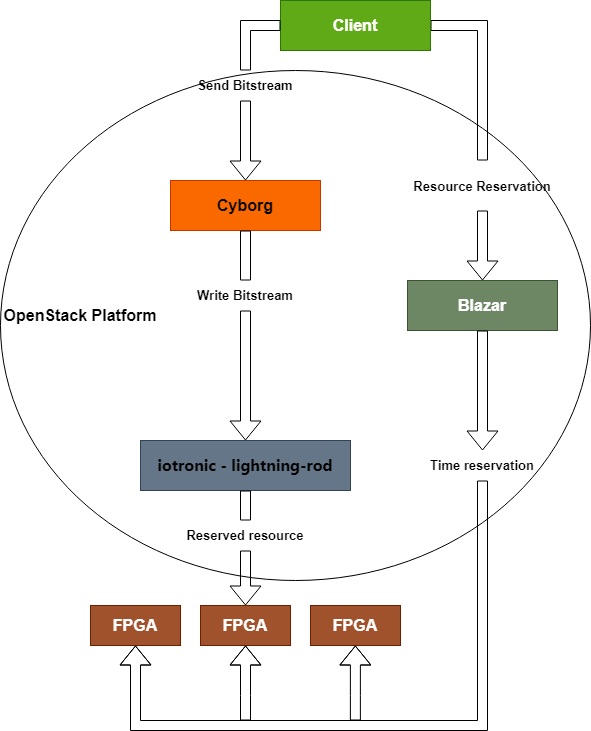
\includegraphics[width=0.5\textwidth]{images/Stack1.png}
\caption{Stack dell'architettura}
\end{figure}\clearpage
L'utente finale vedrà la webpage che si interfaccerà a Blazar tramite delle API le quale gli permetteranno la prenotazione delle risorse.
\begin{figure}[h]
\centering
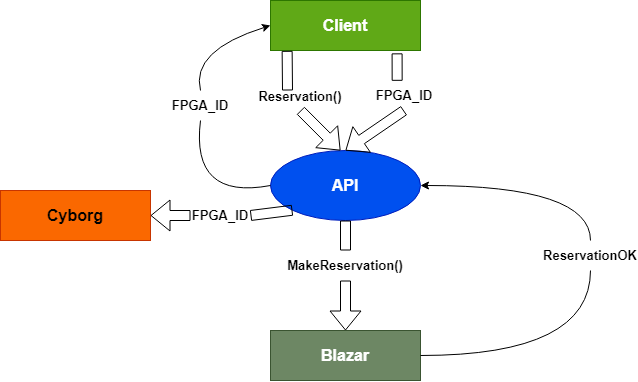
\includegraphics[width=0.7\textwidth]{images/Arch1.png}
\caption{Diagramma che rappresenta le fasi di reservation}
\end{figure}\\
Una volta avvenuta l'effettiva prenotazione l'utente finale sarà in grado tramite le API fornite da Cyborg ed il loro interfacciamento con i driver a bordo della scheda la riprogrammazione tramite bitstream di quest'ultima ed il suo completo utilizzo. 
\begin{figure}[h]
\centering
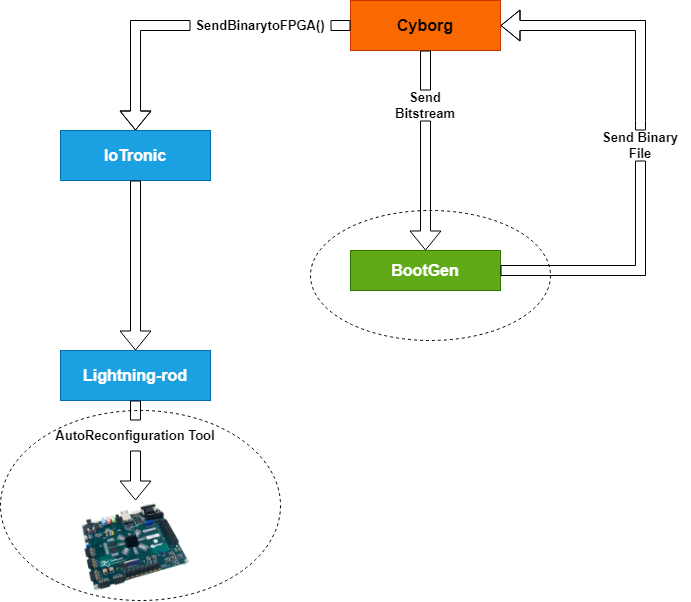
\includegraphics[width=0.7\textwidth]{images/Arch.png}
\caption{Diagramma che rappresenta le fasi post upload del bitstream}
\end{figure}\\
